
\section{Angle dependent measurements}
    \label{Sec:3:AngleDependentMeasurements}


\subsection{Mapping the Fermi surface with DFT calculations}
    \label{Sec:3:MappingFermiSurfaceDFTCalulations}

\begin{figure}[h!]
    \begin{center}
        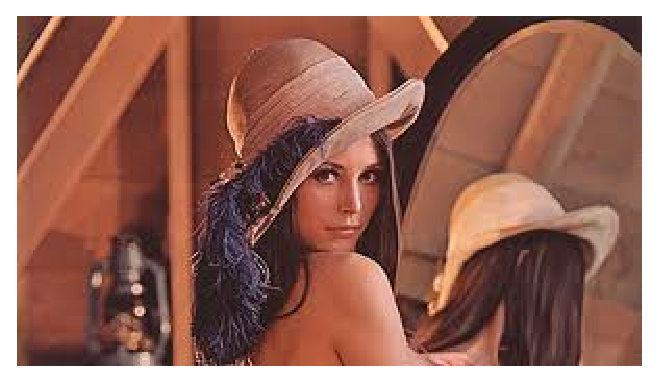
\includegraphics[scale=0.7]{Misc/TODO}
        \caption{dHvA frequencies nultipled by angle of the $B$ field. Solid lines are DFT calculations, open circles are measured data. $B$ field directed along (a) $[001]\rightarrow[100]$ and (b) $[001]\rightarrow[110]$.}
        \label{Fig:3:ComparisonRotationPlotMeasuredDFT}
    \end{center}
\end{figure}


\subsubsection{Rigidly shifting the calculated DFT energies}

As is shown in \fig~\ref{Fig:3:ComparisonRotationPlotMeasuredDFT}, the rotation plots from the DFT calculations match up qualitatively with the data but do not match up quantitatively -- the electron bands overestimating the size of the measured extremal orbits by around TODO and the hole orbits overestimating the extremal orbits by around TODO. 

\begin{figure}[h!]
    \begin{center}
        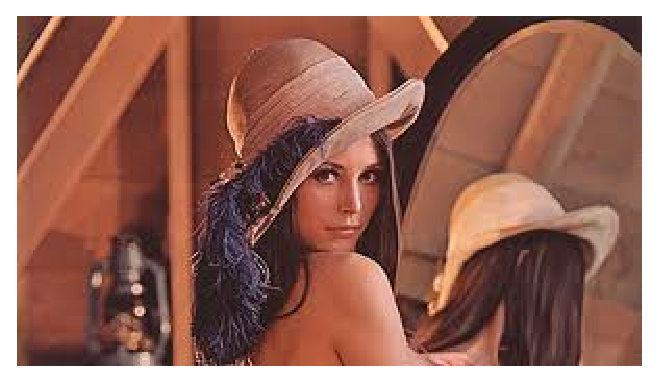
\includegraphics[scale=0.7]{Misc/TODO}
        \caption{dHvA frequencies multipled by the cosine of the angle of the $B$ field. Solid lines are rigidly shifted DFT calculations, open circles are measured data. $B$ field directed along (a) $[001]\rightarrow[100]$ and (b) $[001]\rightarrow[110]$.}
        \label{Fig:3:ComparisonRotationPlotMeasuredShiftedDFT}
    \end{center}
\end{figure}

In order to obtain the correct shape of Fermi surface, the DFT calculations need to be tweaked. One technique is to apply small band-specific rigid energy shifts, which, in most cases is enough to bring the DFT in line with the experimental data. \fig~\ref{Fig:3:ComparisonRotationPlotMeasuredShiftedDFT} shows the rotation plots which rotate towards both the 100 and 110 directions along with appropriately shifted calculations. Table~\ref{Table:3:EnergyShifts} lists those energy shifts.

\medskip

\begin{center}
    \begin{tabular}[h!]{llr}
\toprule
Band    & \multicolumn{2}{l}{Energy Shift (\unit{Ry})} \\
\midrule
1       &       & -0.0083      \\
2       & Wide  & 0.0          \\
        & Narrow & -0.0038     \\
3       &       & 0.0043       \\
4       &       & 0.0050        \\
\bottomrule
    \label{Table:3:EnergyShifts}
    \end{tabular}
\end{center}

Band $2$ in this case has two separate shifts specified in two different regions of the Brillouin zone. The rotation plot for the wider orbit located at the edge of the Brillouin zone was calculated with no energy shift and the narrow part of the Fermi surface around the $\Gamma$ point was calculated with a shift of $0.0038\unit{Ry}$. This provides a reasonable match for the rotation plot where we can apply the shift to the two regions discretely, however is proves problematic when we wish to study intermediate areas since it is not clear how the Fermi surface varies between the two regions.

\subsubsection{Shifting the DFT calculations proptional to orbital character}
\label{Sec:ShiftingDFTPropToOrbitalCharacter}

\Fig~\ref{Fig:3:Band2DCharacter} shows the strength of various d-orbital band characters taken on a 110 cut through the \BaFeP Brillouin zone with the band $2$ Fermi surface superimposed. Band characters for the other bands can be found in Appendix~\ref{TODO}.
%%
\begin{figure}[h!]
    \begin{center}
        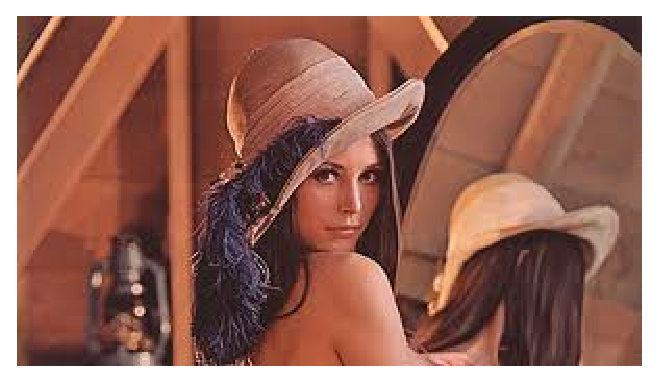
\includegraphics[scale=0.7]{Misc/TODO}
        \caption{Partial $d$-orbital character of the hole band $2$ across slices in the 110 direction. Solid lines show the Fermi surface in the plane.}
        \label{Fig:3:Band2DCharacter}
    \end{center}
\end{figure}
%%
\begin{figure}[h!]
    \begin{center}
        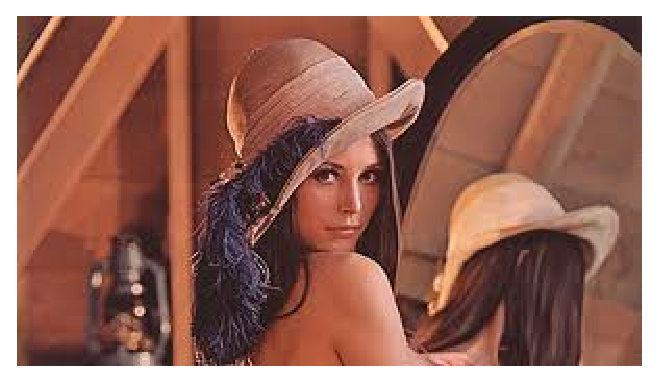
\includegraphics[scale=0.7]{Misc/TODO}
        \caption{Partial $d$-orbital characters of the hole band $2$ along the Fermi surface in the 110 slice vs. \kz}
        \label{Fig:3:Band2DCharacterVsKz}
    \end{center}
\end{figure}

Band $2$ has very little \Dxy and \DxTwoyTwo character close to the Fermi level but shows a significant amount of \DzTwo character at the wide region of the Fermi surface and \DxzDyz character at the narrow region. \Fig~\ref{Fig:3:Band2DCharacterVsKz} shows the orbital character for each of the $d$-orbitals as a function of \kz along the Fermi surface. Evidently, energy shifts could be applied which are scaled to either the \DzTwo and \DxzDyz orbital character in order that we obtain a smooth energy shift transition between the narrow and wide regions discussed previously.

Energy shifts were applied across the full $3$d Brillouin zone for band $2$ using the following two scalings,
%%
\begin{align*}
\textrm{\DzTwo:}\quad \Delta\epsilon &= 0.002 - 0.0052 (1 - (\epsilon - 0.033)/(0.2205 - 0.033)) \\
\textrm{\DxzDyz:}\quad \Delta\epsilon &= 0.002 - 0.0052 (\epsilon - 0.0946)/(0.3135 - 0.0946)
\end{align*}
%%
Note that these scalings ensure that the energy shift applied varies between $-0.0032\unit{Ry}$ and $0.002\unit{Ry}$ which are slightly different to the values applied when rigidly shifting the band. This is due to the fact that the Fermi surface area measured in one region is affected more and more by the size of the Fermi surface in the opposite region as the azimuthal angle gets higher and the calculated area deviates from the measured area. This is what results in the crossing of the calculated rotation plot with the measured rotation plot shown in the first panel of \fig~\ref{Fig:3:Band2DCharacterRigidComparison}. A rigid shift was therefore chosen which best lines up along the length of the curve -- one which will be slightly lower than if we were to match the plots exactly at the 001 direction.

\begin{figure}[h!]
    \begin{center}
        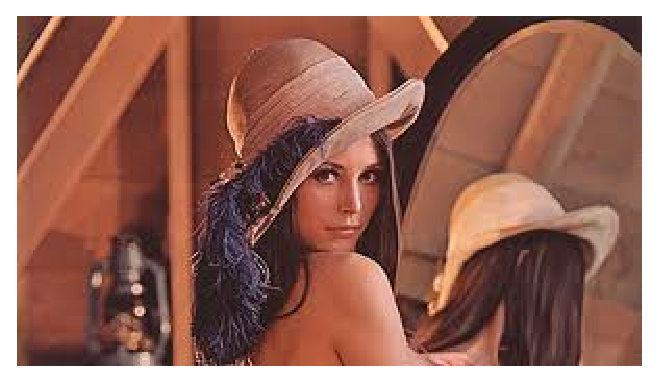
\includegraphics[scale=0.7]{Misc/TODO}
        \caption{dHvA frequencies for band 2 multipled by the cosine of the angle of the $B$ field. $B$ field directed along $[001]\rightarrow[110]$. Open circles are measured data, solid lines represent (a) rigidly shifted DFT calculations, (b) DFT calculations shifted proportional to \DzTwo orbital character, (c) DFT calculations shifted proportional to \DxzDyz orbital character.}
        \label{Fig:3:Band2DCharacterRigidComparison}
    \end{center}
\end{figure}

The second and third panels of \fig~\ref{Fig:3:Band2DCharacterRigidComparison} show the rotation plots calculated with the energy shifts applied proportional to \DzTwo and \DxzDyz orbital character respecitvely. We observe a much better alignment of the measured and calculated data for all angles.






\subsection{Susceptibility calculations}
\label{Sec:SubsceptibilityCalculation}
